\documentclass[10pt,a4paper]{article}
\usepackage[utf8]{inputenc}
\usepackage[german]{babel}
\usepackage[left=1.5cm,right=1.5cm,top=1.5cm,bottom=1.5cm]{geometry}
\author{Andreas Hemmetter}
\let\footruleskip\undefined %undefine footruleskip
\usepackage{fancyhdr}
\usepackage{multicol}
% \usepackage{textcomp}
% \usepackage{amsthm}
\usepackage{framed}
\usepackage{multirow}
\usepackage{xhfill}
% \usepackage{bbold}
% \usepackage{amssymb}
\usepackage{hyperref}
\usepackage{booktabs}
\usepackage{graphicx}
%\usepackage{braket}
% \usepackage{tikz}
% \usetikzlibrary{arrows}
\setlength{\headheight}{15.2pt}
\begin{document}
\pagestyle{fancyplain}
\fancyhf{}
\rhead{\textbf{\textit{Toki Pona}} - \href{mailto:a.hemmetter@gmail.com}{A. Hemmetter} }
\rfoot{\scriptsize{This work is licensed under a \href{https://creativecommons.org/licenses/by-sa/4.0/}{Creative Commons Attribution-ShareAlike 4.0 International License}. Grafik von Bryant Knight (jan Pije).}}
\begin{center}

\begin{tabular}[t]{@{}l}
\rule[4pt]{0.35\linewidth}{4pt}
\end{tabular}
\begin{tabular}[t]{@{}}
\fontsize{24pt}{10pt}
\textbf{Toki Pona}
\end{tabular}
\begin{tabular}[t]{r@{}}
\rule[4pt]{0.35\linewidth}{4pt}
\end{tabular}
\end{center}

\paragraph{Was ist Toki Pona?}
Toki Pona ist eine minimalistische Sprache, erfunden von der kanadischen Linguistin Sonja Lang mit dem Ziel, dem Sprecher zu helfen, seine Gedanken zu vereinfachen. Die Sprache basiert auf der Idee, dass bereits eine kleine Grammatik und Wortschatz für fast jede Kommunikation ausreicht. Stell dir vor du wärst auf einer einsamen Insel mit einer Babel-esken Gruppe von Mitüberlebenden gestrandet - nur mit diesem Zettel und ein wenig Zeit könnt ihr anfangen zu kommunizieren. Zeit habt ihr ja dann sowieso genug. Es ist eine mit Absicht sehr einfach gehaltene Sprache, und es ist von Vorteil auch die Gespräche so zu halten.

\begin{multicols}{2}
\paragraph{Laute und Schrift}

Toki Pona benutzt nur Laute, die in fast jeder Sprache vorkommen. Diese sind  \textbf{k}, \textbf{l}, \textbf{m}, \textbf{n}, \textbf{p}, \textbf{s}, \textbf{t}, \textbf{w} and \textbf{j} als Konsonanten und \textbf{a}, \textbf{e}, \textbf{i}, \textbf{o} und \textbf{u} als Vokale. Erlaubte Silben folgen dem KV(n)-Muster. Es gibt keine Großschreibung, außer bei Eigennamen. Wegen seiner begrenzten Phonologie kann Toki Pona mit praktisch jeder Schrift geschrieben werden, z.B. Hangul, Arabisch, Kyrillisch oder in Hieroglyphen (\textbf{sitelen suwi} oderr \textbf{linja pona}). Mach's einfach, wie du willst.

\paragraph{Wortschatz}

Toki Pona hat einen winzigen Wortschatz von gut 120 Wörtern und ist daher ziemlich mehrdeutig. Wörter haben eine flexible Anzahl, Geschlecht, Funktion im Satz und sogar genaue Bedeutung. Im Prinzip repräsentieren sie \textit{Konzepte} und ihre genaue Bedeutung sollte aus dem Kontext klar werden. Zum Beispiel kann \textbf{mi moku} \textit{Ich esse / Ich werde essen / Ich aß / Ich bin Essen} bedeuten. Präzisere Wörter kann man durch Wortverbindungen ausdrücken, indem man Adjektive \underline{nach} dem Hauptkonzept anhängt: \textbf{jan} [\textit{Person}], \textbf{jan utala} [\textit{kämpferische Person (Soldat)}], \textbf{jan utala nasa} [\textit{dummer Soldat}], etc. Jedes Wort, auch \textbf{mute} [\textit{viele}], \textbf{ni} [\textit{dieses}] und alle Pronomen können auch als Adjektive/Adverben nach einem Substantiv/Verb stehen: \textbf{mi utala ike} [\textit{Ich kämpfe schlecht}]. Daher kommt das Problem (oder Feature, je nach dem wie man das sieht), dass das gleiche Wort für verschiedene Leute unterschiedlich ausgedrückt werden kann: \textit{Kaffee} kann z.B. \textbf{telo pi lape ala} [\textit{Flüssigkeit, die jemanden nicht schlafen lässt}], \textbf{telo wawa pimeja} [\textit{starke, schwarze Flüssigkeit}], \textbf{telo jaki ike} [\textit{ekliges Dreckwasser}], usw. sein. Du siehst ja, was ich meine.

\paragraph{Satzstruktur}

Kleb einfach Wörter aneinander um auszudrücken, was du sagen willst. Falls der Satz zu lang oder kompliziert wird, spalte ihn einfach auf oder lass es einfach. Aber nicht so schnell! Toki Pona braucht die kleinen Schlüsselwörter \textbf{li} um Subjekt und Prädikat (außer direkt nach \textbf{mi} [\textit{ich}] und \textbf{sina} [\textit{du}]) und \textbf{e} um Prädikat vom Objekt zu trennen: \textbf{ona li pona e ilo} [\textit{Sie repariert das Werkzeug}]. Des Weiteren können mehrere \textbf{li} oder \textbf{e} als \textit{und} verwendet werden: \textbf{pipi li lukin li moku} [\textit{Der Käfer schaut und isst}] und \textbf{mi moku e kili e telo} [\textit{Ich esse Früchte und (trinke) Wasser}]. Es gibt kein Verb \textit{sein}, \textbf{mi pona} ist also \textit{Ich bin gut}.

\paragraph{Negation und Fragesätze}

Ein Wort kann verneint werden, indem wir \textbf{ala} [\textit{nicht}] hinter das Verb kleben: \textbf{mi wile ala tawa musi} [\textit{Ich will nicht tanzen}]; im Prinzip funktioniert es wie ein Adjektiv (wie auch \textbf{ali} [\textit{alles}]). Ja/Nein-Fragen formuliert man, indem man das Verb nach \textbf{ala} wiederholt: \textbf{sina pona ala pona?} [\textit{Alles klar bei dir?}]. Als Antwort kann man einfach das Verb mit oder ohne \textbf{ala} wiederholen. Um nach dem Subjekt des Satzes zu fragen, benutzt man \textbf{seme}: \textbf{seme li lon tomo mi?} [\textit{Was ist in meinem Haus?}]. Es kann auch benutzt werden, um nach dem Objekt (\textbf{sina lukin e seme?} [\textit{Was schaust du an?}]), einer Person (\textbf{jan seme li moku?} [\textit{Wer isst?}]), dem Grund (\textbf{sina kama tan seme?} [\textit{Warum bist du gekommen?}]) oder nach einem bestimmten Subjekt/Objekt zu fragen (\textbf{ma seme li pona tawa sina?} [\textit{Welche (der) Länder gefallen dir?}]). Das Wort \textbf{anu} [\textit{oder}] verwendet man nur für die Auswahl zwischen zwei Optionen: \textbf{sina jo e kili anu telo nasa?} [\textit{Ist es eine Frucht oder Wein, was du da hast?}], \textbf{... anu seme?} [\textit{..., nicht wahr?}].
\end{multicols}

\paragraph{Präpositionen}

Präpositionen können auch als Verben, Substantive oder Adjektive fungieren - genau so, wie jedes andere Wort auch - aber benötigen kein \textbf{e} vor dem Objekt. Präpositionen sind \textbf{lon} [\textit{in/bei/auf etwas sein}], \textbf{kepeken} [\textit{etwas benutzen}], \textbf{tawa} [\textit{sich wohin bewegen}], \textbf{kama} [\textit{kommen/verursachen}], \textbf{sama} [\textit{wie}], \textbf{tan} [\textit{weil}] and \textbf{poka} [\textit{neben}]. Verwandt damit sind auch Modalverben (Hilfsverben) wie z.B. \textbf{wile} [\textit{wollen/brauchen}], welche immer direkt vor einem Prädikat stehen (also ohne \textbf{li}).

\begin{multicols}{2}
\noindent\textbf{suno li lon sewi} [\textit{Die Sonne ist im Himmel}]\\
\noindent\textbf{mi wile e ni: mi lon tomo} [\textit{Ich will zuhause sein}]\\
\noindent\textbf{mi tawa tomo mi} [\textit{Ich gehe zu meinem Haus}]\\
\noindent\textbf{mi toki tawa sina} [\textit{Ich spreche mit dir}]\\
\noindent\textbf{ni li pona tawa mi} [\textit{Das ist gut für mich (Ich mag das)}]\\
\noindent\textbf{mi tawa e kiwen} [\textit{Ich bewege den Stein}]\\
\noindent\textbf{ona li kama tawa tomo mi} [\textit{Er kam zu meinem Haus}]\\
\noindent\textbf{mi kama e pakala} [\textit{Ich habe einen Unfall verursacht}]\\
\noindent\textbf{mi kama jo e telo} [\textit{Ich hole Wasser}]\\
\noindent\textbf{mi moku kepeken ilo moku} [\textit{Ich esse mit einer Gabel/Löffel/Stäbchen}]\\
\noindent\textbf{mi kepeken e poki} [\textit{Ich benutze eine Tasse}]\\
\noindent\textbf{mi moku poka jan pona mi} [\textit{Ich esse bei meinem Freund}]\\
\noindent\textbf{jan ni li sama mi} [\textit{Diese Person ist wie ich}]\\
\noindent\textbf{mi moku tan ni: mi wile moku} [\textit{Ich esse, weil ich Hunger habe}]\\
\noindent Andere Wörter, die wie Präpositionen funktionieren:\\
\noindent\textbf{ona li lon sewi mi} [\textit{Er ist über mir}]\\
\noindent\textbf{pipi li lon anpa mi} [\textit{Der Käfer ist unter mir}]\\
\noindent\textbf{moku li lon insa mi} [\textit{Essen ist in meinem Bauch}]\\
\noindent\textbf{len li lon poka mi} [\textit{Die Kleider liegen neben mir}]
\end{multicols}

\paragraph{Dinge, die man nicht so genau sagen muss}
Farben drückt man als Mischungen/Töne von den fünf Grundfarben aus: \textbf{jelo} [\textit{gelb}], \textbf{laso} [\textit{blau}], \textbf{loje} [\textit{rot}], \textbf{pimeja} [\textit{schwarz}] and \textbf{walo} [\textit{weiß}]. Aber übertreib's nicht: die genaue Farbe einer Banane ist unwichtig; es ist halt einfach eine \textbf{kili palisa jelo}.\\
\noindent Es gibt kein richtiges System um große, präzise Zahlen auszudrücken, da man es fast immer vermeiden kann, und weil sonst der ganze Spaß an der Sprache (Vereinfachung unserer Gedanken) flöten geht. Jetzt, wo das aus dem Weg ist, wird man feststellen, dass es trotzdem vier Zahlen gibt, die man zu größeren zusammensetzen kann:\textbf{ala} [\textit{null}], \textbf{wan} [\textit{eins} oder \textit{verbinden}], \textbf{tu} [\textit{zwei} or \textit{teilen}] und \textbf{luka} [\textit{fünf}]. Diese Wörter kann man addieren um größere Zahlen zu bekommen (\textbf{luka tu wan} [\textit{acht}]), aber am besten benutzt man einfach \textbf{mute} [\textit{viele}] für alles andere. Genaue Mengen tragen meistens nichts zum Gespräch bei. Versuch einfach ohne diese auszukommen.\\
Falls es absolut notwendig ist, kann man Zeiten durch \textbf{tenpo pini la ...} (Vergangenheit), \textbf{tenpo ni la ...} (Gegenwart) and \textbf{tenpo kama la ...} (Zukunft) kennzeichnen. Das gleiche gilt für das Geschlecht eines Wortes, bei dem man die Adjektive \textbf{meli} [\textit{weiblich}] und \textbf{mije} [\textit{männlich}] benutzt.

\paragraph{Details}
\begin{multicols}{2}
\begin{itemize}
\item Ortsnamen sind immer Adjektive und gehorchen den Silbenregeln in Toki Pona: \textbf{ma Kanata} [\textit{(das Land) Kanada}]. Das gleiche gilt für Sprachen (\textbf{toki}), Nationalitäten (\textbf{jan}), Namen (\textbf{jan}), usw.
\item Den Imperativ macht man, indem man ein \textbf{o} vor das Verb schiebt: \textbf{o pali!} [\textit{Arbeite!}]. Die Anrede funktioniert mit einem \textbf{o} hinter dem Namen: \textbf{jan Keli o, sina pona lukin} [\textit{Kelly, die siehst gut aus!}]. Falls Anrede und Imperativ im gleichen Satz sind, kann man ein \textbf{o} weglassen.
\item Das Wort \textbf{pi} [\textit{von}] \underline{teilt} Bedeutungen: \textbf{tomo telo nasa} [\textit{komische Toilette}], \textbf{tomo pi telo nasa} [\textit{Haus des Alkohols (Bar)}]. Es kann auch den Besitzer spezifizieren: \textbf{tomo pi jan Lisa} [\textit{Lisas Haus}].
\item Wir können \textbf{taso} [\textit{aber/doch}] benutzen, um inhaltlich verwandte Sätze zusammen zu schnüren.
\end{itemize}
\end{multicols}

\begin{center}
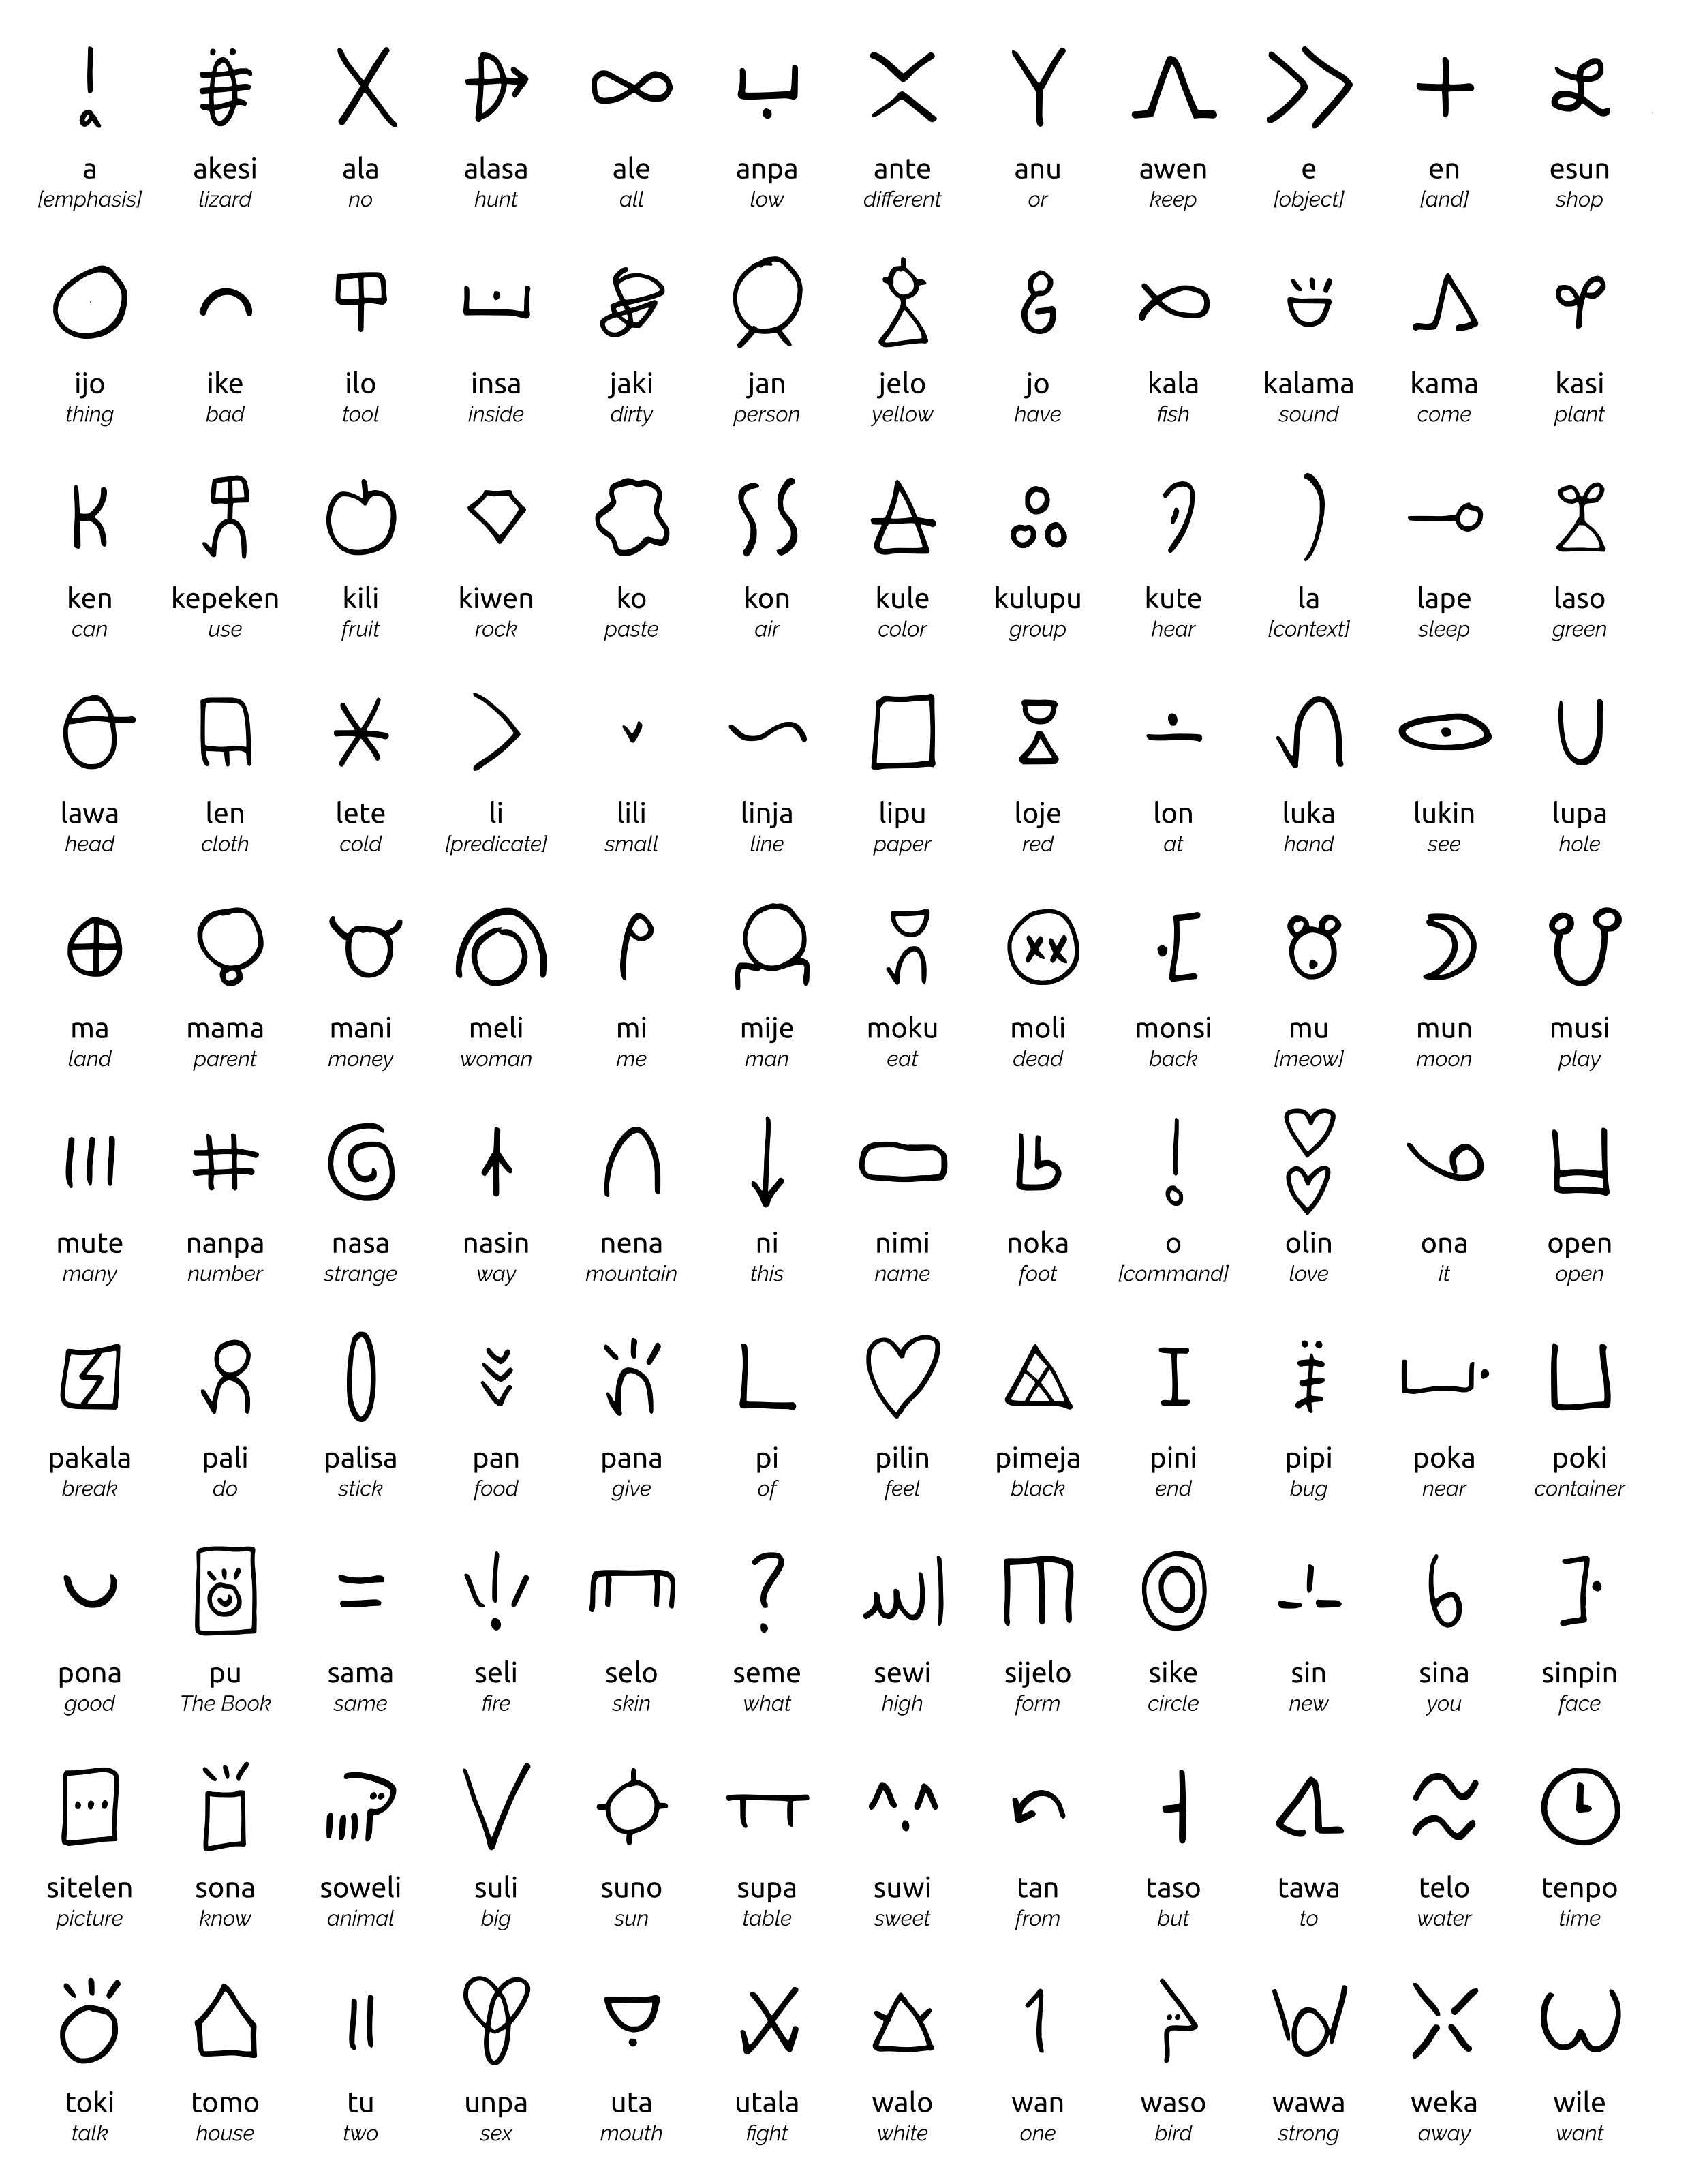
\includegraphics[width=0.75\linewidth]{tokipona.png}
\end{center}
\end{document}
